%%% Ne pas modifier jusqu'à la ligne 25
\documentclass[a4paper,12pt]{book}
\usepackage[utf8]{inputenc}
\usepackage[french]{babel}
%%\usepackage{CJK}
\usepackage{yhmath}
\usepackage[left=2cm,right=2cm,top=3cm,bottom=2cm, headheight=1.5cm,headsep=1.5cm]{geometry}
%%\usepackage{CJKutf8}
\usepackage{amsfonts}
\usepackage{mathrsfs}
\usepackage{amsmath,amsfonts,amssymb,dsfont}
\usepackage{graphicx}
\usepackage{subfigure}
\usepackage{enumitem}		%\enumerate-resume
\usepackage[colorlinks=true,unicode={true},hyperindex=false, linkcolor=blue, urlcolor=blue]{hyperref}
\newcommand{\myref}[1]{\ref{#1} page \pageref{#1}}

\addto\captionsfrench{\def\tablename{Tableau}}  %légendes des tableaux
\renewcommand\thesection{\Roman{section}~-~} 
\renewcommand\thesubsection{\Roman{section}.\Alph{subsection}~-~} 
\renewcommand\thesubsubsection{\Roman{section}.\Alph{subsection}.\arabic{subsubsection}~-~} 

\newcommand{\conclusion}[1]{\newline \centerline{\fbox{#1}}}

\setcounter{secnumdepth}{3}
\parindent=0pt

\usepackage{fancyhdr}
\pagestyle{fancy}

\lhead{SJTU-ParisTech} 
%%%%%%%%%%%%%%%%%%%%%%%%%%%%%%%%%%
\chead{DM5}
\rhead{Daniel 518261910024}

\begin{document}
\renewcommand{\labelitemi}{$\blacktriangleright$}
\renewcommand{\labelitemii}{$\bullet$}


\section{Exercice 5-1}
\begin{itemize}
    \item système: $(\Sigma)$: Le plateau de masse M et de rayon R et l'homme de masse m
    \item référentiel: référentiel terrestre $(R)$ supposé galiléen, référentiel lié à le plateau $(R_1)$, référentiel lié à l'homme $(R_2)$
    On a $\overrightarrow{\Omega}_{(R_1)/R}=\dot{\theta} \vec{e_z}$, et $\overrightarrow{\Omega}_{(R_2)/R}=\dot{\varphi} \vec{e_z}$
\end{itemize}
\begin{figure}[h]
    \begin{center}
    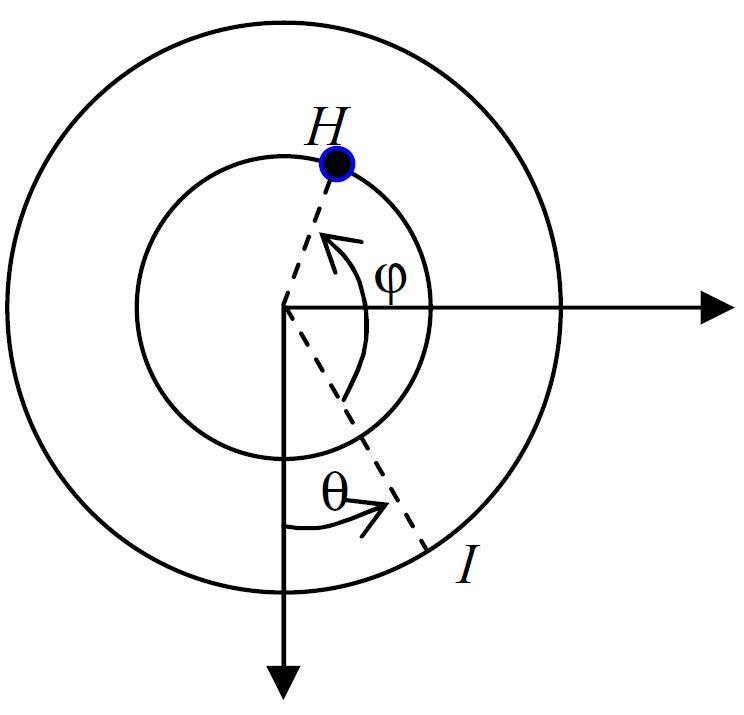
\includegraphics[scale=2]{meca5.jpg}
    \end{center}
    \caption{le système étudiée}
\end{figure}
\subsection{}
Comme le plateau tournersans frottement autour d'un axe, on a donc $\overrightarrow{\mathcal{M}}_{\Delta,ext \to (\Sigma)}=\vec{0}$, 
par le théorème scalaire du moment cinétique, on a 
$$
\left(\frac{dL_\Delta(\Sigma)}{dt}\right)_{(R)}=\mathcal{M}_{\Delta,ext \to (\Sigma)}=0
$$
le moment cinétique total par rapport à l'axe est donc conservé
\subsection{}
Comme 
$$
L_\Delta(\Sigma)=L_1+L_2 
$$
avec
$$
L_1=I_1\Omega_1=ma^2\dot{\varphi} \quad
\mbox{et} \quad
L_2=I_2\Omega_1=\frac{1}{2}MR^2\dot{\theta}
$$
Donc 
$$
\frac{d}{dt}\left(ma^2\dot{\varphi}+\frac{1}{2}MR^2\dot{\theta}\right)=0
$$
Soit
$$
ma^2\ddot{\varphi}+\frac{1}{2}MR^2\ddot{\theta}=0
$$
On obtient
$$
\ddot{\varphi}=-\frac{MR^2}{2ma^2}\ddot{\theta}
$$
En intégrant, avec les conditions initiales $\dot{\varphi}(t=0)=\dot{\theta}(t=0)$, on obtient
$$
\dot{\varphi}=-\frac{MR^2}{2ma^2}\dot{\theta}
$$
Donc 
$$
2\pi=[\varphi(t=t_f)-\varphi(t=0)]-[\theta(t=t_f)-\theta(t=0)]=\left(-\frac{MR^2}{2ma^2}-1\right)(\theta(t=t_f)-\theta(t=0))
$$
Finalemant, le disque a tourné $\boxed{\Delta \theta=-\frac{2\pi }{1+\frac{MR^2}{2ma^2}}}$
\subsection{}
A.N. 
$$
\boxed{\Delta \theta=-\frac{2*3.14}{1+\frac{500*9}{2*75*1}}=-0.203}
$$
Le plateau a peu tourné par rapport l'homme




\end{document}